\section{Analysis}
In this section, we present the analysis of the obtained data. The structure of the analysis is as follows: We start 
of with analyzing the monochromator. To this end, we investigate its calibration with the Hg-lamp's peaks, examine 
the influence of the slit width, identify the upper boundary of detection (in terms of wavelength) and measure the 
different detection probabilities for vertically and horizontally polarized light. 
Then we visualize the measured spectrum overviews of three samples, carbon disulfide (CS$_2$), chloroform (CHCl$_3$),
and carbon tetrachloride (CCl$_4$) and identify visible Stokes 
and Anti-Stokes peaks. The data is of rather bad quality, having a low signal-to-noise ratio. Especially under the given 
time constraints, we were not able to obtain better signals by adjusting the accessible experimental parameters. We 
therefore have to refrain from doing further analysis with these spectra. 

Instead, we decided to do the bulk of the analysis on data taken by the CCD spectrometer. The corresponding second part 
of the analysis follows a similar structure. We start of by verifying the calibration of the CCD spectrometer with the 
Hg-lamp, continued by the sensitivity analysis regarding polarized light with a resulting correction factor. Proceeding 
differently to the prior analysis, we go on by investigating the laser used in the experiment. Then we examine the 
properties of the notch filter used in all of the spectra later on. This is done in a qualitative manner since there was 
no possibility of changing the parameters of this part of the experiment. 

The most important part of the analysis comes at this point: The analysis of the spectra of all samples at hand. For 
the first two, CS$_2$, CHCl$_3$, we only fit all visible peaks and compare the results to literature values. The following 
samples, however, are each used to highlight as specific aspect connected to Raman spectroscopy. The CCl$_4$ sample is 
used to demonstrate the effects of asymmetry in the molecule, resulting in a depolarization of the scattered light. The 
linear dependence of the intensity of Raman peaks on the concentration of the corresponding substance is used to measure 
the concentration of ethanol in an unknown ethanol-water mixture, highlighting a widely used application of Raman 
spectroscopy for characterizing unknown substances. And a final analysis of a measurement of sulfur is used to measure the 
temperature of the probe. Although of questionable reliability, this last part demonstrates the theoretical connection 
between the experiment and results of statistical mechanics. 

The literature values in this section, namely the wavenumbers of various peaks, are taken from the NIST 
Computational Chemistry Comparison and Benchmark DataBase\cite{nist}. 

\subsection{Monochromator}
The data taken with the monochromator is closely connected to the experimental setup. Many parameters were accessible 
experimentally and had to be tuned in order to get reasonable results. We will not use all measurements taken, but only 
rely on those with the most usable results. In general, the resolution of the data is restricted by the program used for 
the recordings: Data points are separated by 0.1 nm, regardless of scanning speeds (which could be lowered down to 0.05 
nm / s). This makes fitting impossible in all cases, even in absence of noise (as for the Hg-lamps spectrum). We thus 
identify peaks by searching for local maxima in manually specified regions. The error is estimated rather generously with 
0.2 nm, twice the resolution. One has to keep in mind another source of error, namely the problem of getting the correct 
starting point for a measurement: The registration of data from the monochromator starts once the counter is moving.
However, the starting point has to be set separately for the computer and the device, inducing a possible error of ca. 
0.1 nm for each measurement. 

\subsubsection{Calibration}
The Hg-lamp's spectrum was measured with a $INSERT SPECIFICATIONS HERE: speed, slit width, $ over a range from 400 to 
600 nm. The result is plotted in figure \ref{fig:mono_calibration_hg}. The six observable peaks are found in the
literature -- a comparison is shown in table \ref{tab:mono_calibration}. Due to the good agreement, we go without a linear 
fit and use the values for the wavelength given in the original data in the following analysis. The error induced is 
negligible in comparison to the resolution and offset possibly induced each time. 
\begin{table}[htpb]
    \centering
    \caption{
        Peaks of Hg-spectrum. Notice the good agreement. This is further quantified in a linear regression. 
        }
    \label{tab:mono_calibration}
    \begin{tabular}{c r r}
        \rowcolor{LightCyan} Peak & $\lambda_\text{a} \,/\, \text{nm}$ & $\lambda_\text{lit} \,/\, \text{nm}$ \\
        \cellcolor{LightCyan}$1$ & $404.6 \pm 0.2$ & $404.7$   \\
        \cellcolor{LightCyan}$2$ & $407.7 \pm 0.2$ & $407.8$   \\
        \cellcolor{LightCyan}$3$ & $435.8 \pm 0.2$ & $435.8$   \\
        \cellcolor{LightCyan}$4$ & $546.0 \pm 0.2$ & $546.1$   \\
        \cellcolor{LightCyan}$5$ & $576.9 \pm 0.2$ & $577.1$   \\
        \cellcolor{LightCyan}$6$ & $579.1 \pm 0.2$ & $579.1$ 
    \end{tabular}
\end{table}
\begin{figure}[htpb]
    \centering
    \includegraphics[width=0.8\linewidth]{analysis/figures/mono_calibration_hg.eps}
    \caption{Spectrum of Hg-lamp recorded with the monochromator. The six visible peaks are identified and compared 
    to literature values in order to verify the calibration of the device.}
    \label{fig:mono_calibration_hg}
\end{figure}

\subsubsection{Influence of slid with}
In order to examine the effect of varying the slit width at the entrance of the monochromator, we took measurements of a 
single peak, the 404.7 nm peak of the Hg-spectrum, for width ranging from 25 to 200 $\mu$m. The effects are shown in 
figure \ref{fig:mono_slit}. One observed reducing intensities and widths of the peak. Further, a small effect on the 
center position of the peak is seen: For a 200 $\mu$m opening, the center of the peak is some 0.2 nm higher then for peaks 
between 150 and 40 $\mu$m. The smallest opening yields again yields a slightly higher peak center. These deviations should 
not be overinterpreted, because they might also be due to the described possible fluctuations. The yield of this analysis 
was that we stipulated the width at 100 $\mu$m for the following measurements. 

\begin{figure}[htpb]
    \centering
    \includegraphics[width=0.8\linewidth]{analysis/figures/mono_slit.eps}
    \caption{Effects of slit width of monochromator. Shown are various measurements of the same peak of the Hg-lamp's
    spectrum. The legend indicates the adjusted slid widths, ranging from 200 $\mu$m down to 25 $\mu$m. The effect 
    on the peaks position is well within the expected fluctuations due to difficulties in the setup. The chosen 
    width for further measurements is 100 $\mu$m. }
    \label{fig:mono_slit}
\end{figure}

\subsubsection{Boundary of detection}
The monochromator has only a limited range in which intensities at two different wavelength can be compared directly. Also 
we are not equipped to measure the invariance within the regime (one would need a light source of known intensity 
distribution), we can at least find a upper boundary in terms of wavelength. In order to do so, we assume the white light 
in the experiment to emit radiation following the intensity distribution of black-body radiation. We then compare this 
characteristic distribution with the intensity measured with the white light as the only light source. The measured counts 
at each wavelength are displayed in figure \ref{fig:mono_bound}. One clearly observes a drop in count numbers for 
wavelength above 690 nm. The drop is not abrupt but follows an exponential decay. 
However, without further quantifying the effect, one should not work with data in this regime when concerned about 
intensity. 

\begin{figure}[htpb]
    \centering
    \includegraphics[width=0.8\linewidth]{analysis/figures/mono_bound.eps}
    \caption{Spectrum of the white light on semi log scale recorded with the monochromator and the CCD spectrometer. 
        The decay in counts for wavelengths above 590 (dotted line) indicates the upper boundary of detection for the
    monochromator. The spectrum recorded with the CCD is rescaled for comparability. }
    \label{fig:mono_bound}
\end{figure}

\subsubsection{Detection probability for polarized light}  
Even though the measured spectra do not allow for a detailed analysis including the intensities of the peaks, we still 
measure the detection probability of the monochromator for light polarized vertically or horizontally. We used the white 
light, which is not polarized, and a polarization filter with the angle measured towards the vertical line. The measured
counts (see figure \ref{fig:mono_polarized}) show interesting features: First of all, the detection probability differs by 
a considerable amount for large parts of the range tested. For wavelengths below 500 nm, vertically polarized light is 
detected more easily, above 550 nm the situation is reverted. Further one can observe a step at 430 nm for horizontally 
polarized light, indicating a possible malfunction of the device. To make more precise statements, these features would 
have to be analyzed in a more rigorous manner. 

\begin{figure}[htpb]
    \centering
    \includegraphics[width=0.8\linewidth]{analysis/figures/mono_polarized.eps}
    \caption{Spectrum of white light with polarization filter obtained with the monochromator for two perpendicular 
    polarizations. One observes the dependency on polarization and wavelength for the detection probability. Note further 
    the step at $\lambda = 430$ nm, an unexpected feature not explained by the white light's spectrum. }
    \label{fig:mono_polarized}
\end{figure}

\subsubsection{Spectra of CS$_2$, CHCl$_3$, CCl$_4$}
The spectra of the three samples are measured under slightly varying conditions -- a remainder of our attempts to 
optimize the measurements with the monochromator. Although the original attempt (get signals usable for a quantitative 
analysis including intensity measurements) failed, we did see some peaks which are compared to the literature values in 
the following. Some parameters, however, did not change during these measurements: The slit width was left at 100 $\mu$m, 
the laser was always operated at a current of 1.5 A and we used the $\lambda / 2$ plate to turn the laser's polarization 
by $90^\circ$. Notch filter and polarization filter were not in use. 

The spectrum of carbon disulfide is shown in figure \ref{fig:mono_cs2}. We measured with a sampling speed of 
$0.05$ \AA/s and a voltage of 1000 V applied to the photomultiplier. 
The Rayleigh peak at the laser wavelength of 532 nm is not shown fully because its intensity (1.2e7 counts) 
lies two orders of magnitude above the Stokes peak's intensity.
The latter is found at $551.3 \pm 0.2$ nm, which yields a wavenumber of $653 \pm 14 \text{ cm}^{-1}$ for the respective
vibrational mode.%
\footnote{
    To calculate the wavenumber, we use a laser wavelength of $532.1 \pm 0.3$ nm, an anticipated result of the analysis
    done with the CCD, see section \ref{sec:laser}.
} The literature value of this vibrational mode is $658 \text{ cm}^{-1}$, which is covered quite well within the error.   

\begin{figure}[htpb]
    \centering
    \includegraphics[width=0.8\linewidth]{analysis/figures/mono_cs2.eps}
    \caption{Spectrum of carbon disulfide recorded with the monochromator. Only one Stokes peak is visible (highlighted).
    Background rate as well a noise are abundant. }
    \label{fig:mono_cs2}
\end{figure}


For chloroform (CHCL$_3$) we applied 1000 V to the photomultiplier and sampled with 0.1~\AA/s. The result can be seen in 
figure \ref{fig:mono_chcl3}. Three Stokes peaks are found. Their wavelength and -numbers as well as literature values are 
displayed in table \ref{tab:mono_chcl3}. Especially for the first two peaks, the agreement with the literature is good. 
The last peak is off by more than one standard deviation which shows the strong limitations on our data. Since the 
literature values lack specifications on the intensity of each peak, we cannot derive further conclusions from that
direction either. 

\begin{figure}[htpb]
    \centering
    \includegraphics[width=0.8\linewidth]{analysis/figures/mono_chcl3.eps}
    \caption{Spectrum of chloroform -- overview. The Rayleigh peak is cut off in order to make visible the less obvious 
    features. Three Stokes peaks are visible (highlighted), even though the signal-to-noise ratio is not satisfying.}
    \label{fig:mono_chcl3}
\end{figure}

\begin{table}[htpb]
    \centering
    \caption{
        Stokes peaks for chloroform. 
        }
    \label{tab:mono_chcl3}
    \begin{tabular}{l r r r}
        \rowcolor{LightCyan} Peak N$^o$ & $\lambda \, / \, \text{nm}$ &
        $\Delta \nu \, / \, \text{ cm}^{-1}$ & 
        $\Delta \nu_\text{lit} \, / \, \text{ cm}^{-1}$ \\
        \cellcolor{LightCyan}$1$ & $539.5 \pm 0.2$ & $257 \pm 11$ & $260$   \\
        \cellcolor{LightCyan}$2$ & $542.5 \pm 0.2$ & $360 \pm 11$ & $366$   \\
        \cellcolor{LightCyan}$3$ & $551.6 \pm 0.2$ & $664 \pm 11$ & $680$  
    \end{tabular}
\end{table}

The third spectrum measured with the monochromator is that of carbon tetrachloride (CCl$_4$) and is shown in figure 
\ref{fig:mono_ccl4}. Here we display a measurement done with a much lower voltage applied to the photomultiplier, 
namely 679~V. The sampling speed was again 0.1~\AA/s. One can immediately notice the much lower count rates, both for 
the background and the signals. However, the signal-to-noise ratio does not change considerably. By eye, we identify 
three Stokes and on Anti-Stokes peak. The result of the quantitative analysis is shown in table \ref{tab:mono_ccl4}. 
All four peaks cover the literature values within their error.

\begin{figure}[htpb]
    \centering
    \includegraphics[width=0.8\linewidth]{analysis/figures/mono_ccl4.eps}
    \caption{Overview over spectrum of CCl$_4$ taken with the monochromator. Note the much lower count numbers due to 
    the reduces voltage at the photomultiplier (679 V instead of the previously used 1000 V). Signal-to-noise ratio is 
    not considerably reduced. However, four Raman peaks are visible (highlighted). }
    \label{fig:mono_ccl4}
\end{figure}

\begin{table}[htpb]
    \centering
    \caption{
        3 Stokes and one Anti-Stokes peak for carbon tetrachloride. 
        }
    \label{tab:mono_ccl4}
    \begin{tabular}{l r r r}
        \rowcolor{LightCyan} Peak N$^o$ & $\lambda \, / \, \text{nm}$ &
        $\Delta \nu \, / \, \text{ cm}^{-1}$ & 
        $\Delta \nu_\text{lit} \, / \, \text{ cm}^{-1}$ \\
        \cellcolor{LightCyan}$1$ & $525.9 \pm 0.2$ & $222 \pm 12$ & $217$   \\
        \cellcolor{LightCyan}$2$ & $538.2 \pm 0.2$ & $212 \pm 12$ & $217$   \\
        \cellcolor{LightCyan}$3$ & $541.0 \pm 0.2$ & $309 \pm 11$ & $314$   \\
        \cellcolor{LightCyan}$4$ & $545.5 \pm 0.2$ & $461 \pm 11$ & $459$ 
    \end{tabular}
\end{table}

